\chapter{Exploratory Analysis}
First part of the analysis is to explore the different attributes in the data in order to detect possible patterns or correlations. The exploratory analysis is also used to get an understanding of data and its behaviour. Hence, this chapter is about visualizing the different attributes focusing on their influence on the heat consumption. \textcolor{red}{Mangler nok noget lidt mere her.}

To get an overview of the heat consumption for each house, the daily average consumption for each house has been calculated and can be seen as a function of the time in the following figure. 
\begin{figure}[H]
    \centering
    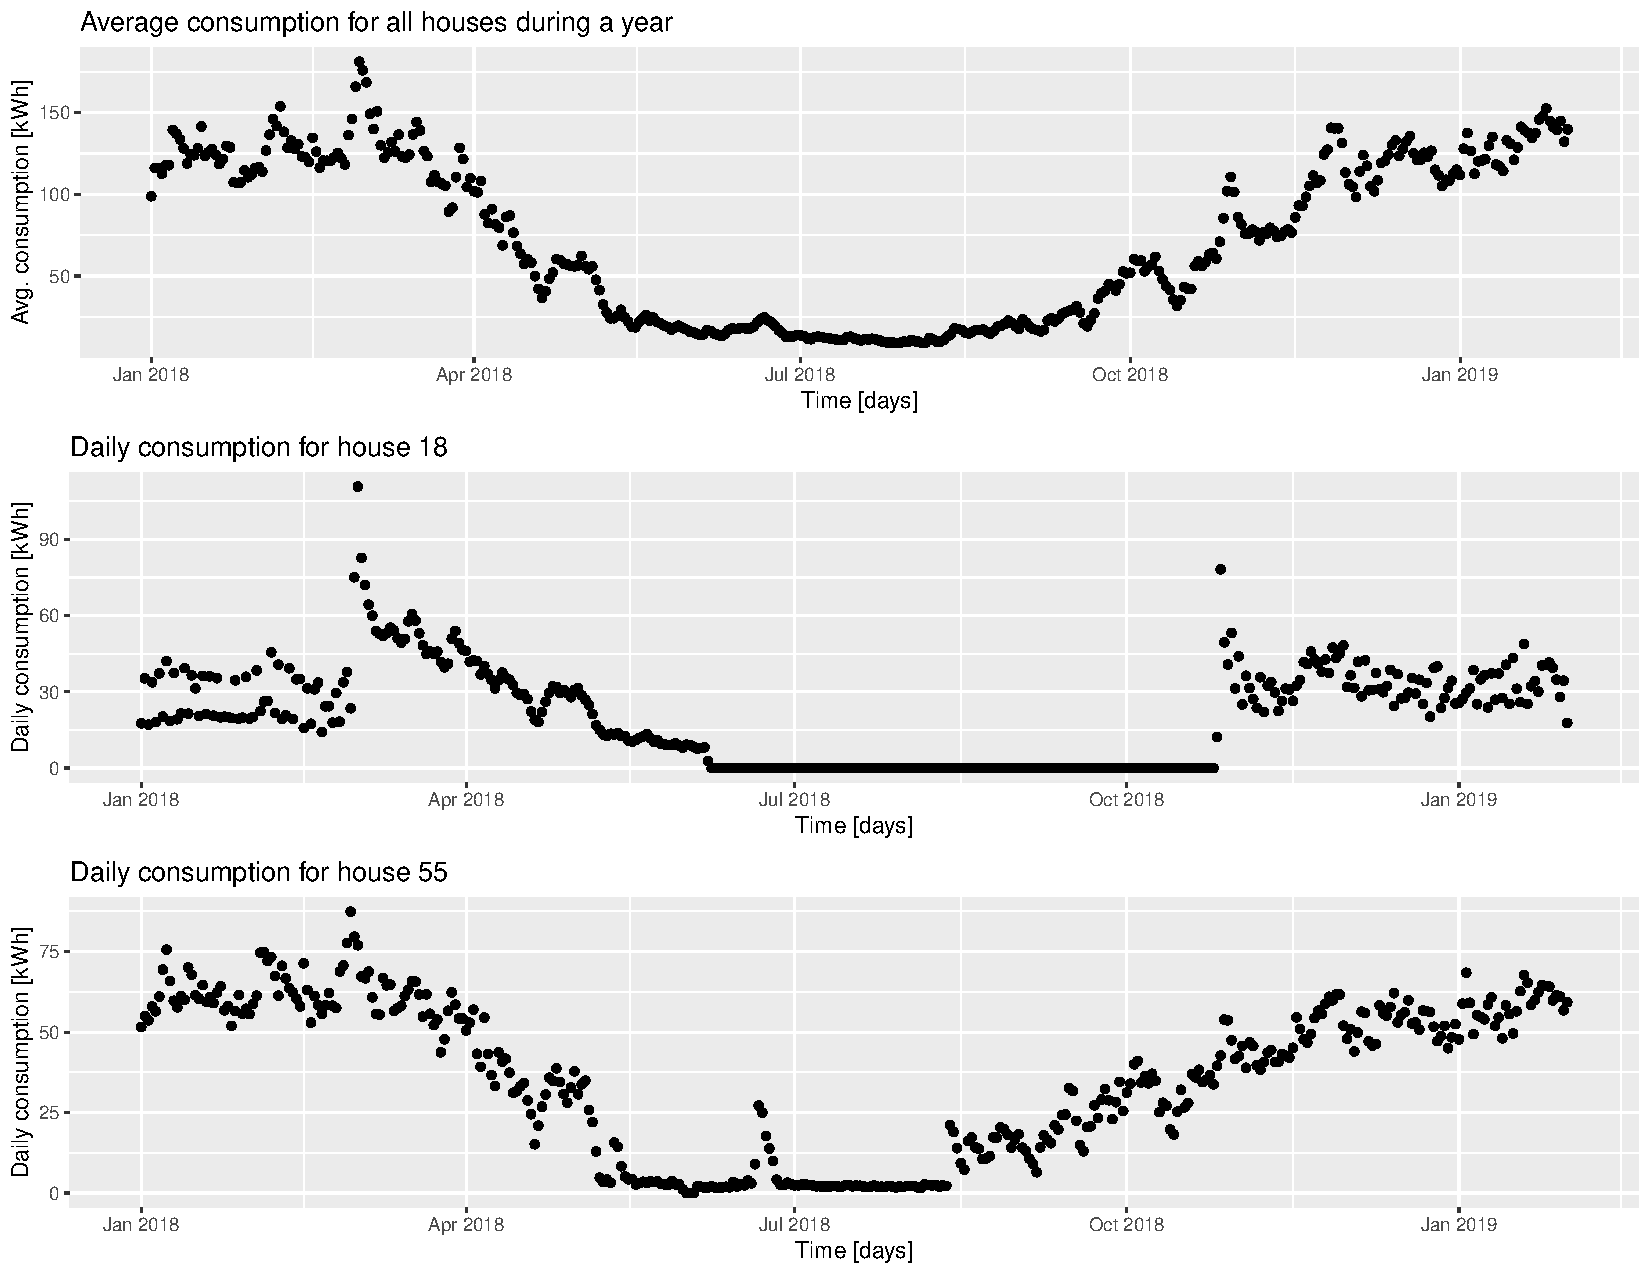
\includegraphics[width=.75\textwidth]{../../../figures/daily_cons.pdf}
    \caption{Daily consumption during a year (2018). The top plot shows the average consumption for all the houses. The plot in the middle shows an example of a house that follows the trend and the last plot shows a house that deviates from the trend.}
    \label{fig: daily_cons}
\end{figure}
Figure \ref{fig: daily_cons} shows the daily average consumption for all the house and the daily consumption of two houses - one that follows the trend at one that deviates. It can be seen that the slopes around the summer months are close to 0. \textcolor{red}{Noget med at vi kun er interesserede i perioden, hvor der er tændt for varmen, så derfor fjerner vi perioden hvor consumption er tæt på 0.} All three plots show some unusual high data points around April 2018. This can be due to the fact that is was snowing \textcolor{red}{blabla}. \\

The average of the attributes from the house data is examined through a scatterplot in order to find possible correlations.
\begin{figure}[H]
    \centering
    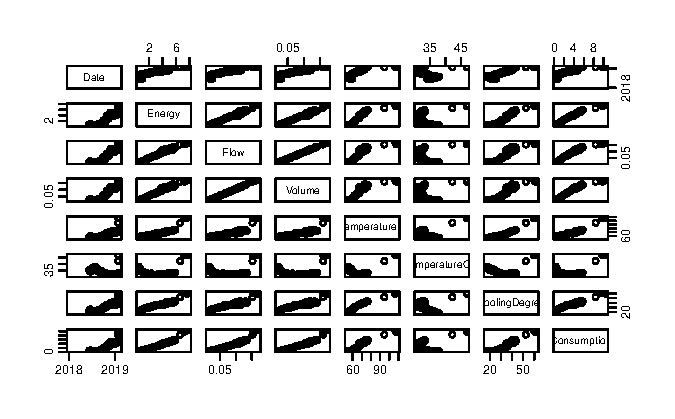
\includegraphics[width=.75\textwidth]{../../../figures/house_attri.pdf}
    \caption{}
    \label{fig: house_attri}
\end{figure}
Figure \ref{fig: house_attri} clearly shows that the consumption is close to 0 in the summer period. 
\textcolor{red}{Pairs af gennemsnitlig house data - vi ser en masse sammenhænge mellem de forskellige attributer. Vi kan se at CoolingDegree skal være over 25, før at varmeforbruget stiger.}
\textcolor{red}{CoolingDegree begynder at stige et stykke tid før flowet stiger, hvilket hænger godt sammen med at når man fx tænder en radiator så stiger CoolingDegree. De efterfølgende radiatorer man tænder øger volumnet.} \\

\begin{figure}[H]
    \centering
    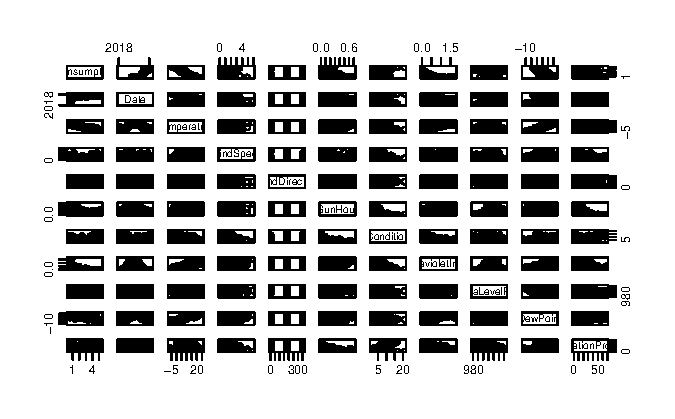
\includegraphics[width=.75\textwidth]{../../../figures/weather_cons_focus.pdf}
    \caption{}
    \label{fig: weather_cons_focus}
\end{figure}

The figure (de udvalgte weather pairs) shows the dependencies between the average consumption of the houses and the weather attributes.
We already know that there is a dependency between the consumption and the time of year. During the summer period there
is almost no consumption. The consumption in this period is probably mostly tap water. The next important thing is the relation
between temperature and consumption. High temperatures tend to imply a higher consumption. And the reason why the consumption
depends so clearly on the time of year can be assumed to that certain periods have similar temperature levels. 
It can also be seen that there is a correlation between dewpoint and consumption. This can be due to the correlation between dewpoint and temperature. \textcolor{red}{Anton nævnte noget med SunHour og Ultravioletindex.}

Figures \ref{fig: house_attri} and \ref{fig: weather_cons_focus} are used to investigate linear relationships which is desired when modelling. If a linear relation is not \textcolor{red}{obtained} this could give rise to a transformation on either the dependent or the independent variable.  